\documentclass[ecp,tc,english]{iiufrgs}
% 
% Outras Opções:
% * english    -- para textos em inglês
% * openright  -- Força início de capítulos em páginas ímpares (padrão da
% biblioteca)
% * oneside    -- Desliga frente-e-verso
% * nominatalocal -- Lê os dados da nominata do arquivo nominatalocal.def


\usepackage[utf8]{inputenc}   % pacote de acentuação unicode
\usepackage{graphicx}         % pacote de importar figuras
\usepackage{times}            % pacote de fonte Adobe Times
% \usepackage{palatino}
% \usepackage{mathptmx}       % pacote de fonte Adobe Times nas fórmulas
\usepackage{fixmath}          % pacote de math international standardization
\usepackage[alf,abnt-emphasize=bf]{abntex2cite}	% pacote de citações abnt


\title{User sessions content-based identification, considering multiple accounts}

\author{Tura}{Matheus Toazza}
\advisor[Prof.~Dr.]{Cordeiro}{Weverton Luis da Costa}
\coadvisor[Prof.~Dr.]{Galante}{Renata de Matos}
\location{Porto Alegre}{RS}
\date{May}{2021}

\keyword{Dimensionality reduction}
\keyword{clustering}
\keyword{user profiling}
\keyword{session identification}
\keyword{recommendation systems}

%\settowidth{\seclen}{1.10~}

\begin{document}

\maketitle

% dedicatoria
% \clearpage
% \begin{flushright}
%     \mbox{}\vfill
%     {\sffamily\itshape
%       ``If I have seen farther than others,\\
%       it is because I stood on the shoulders of giants.''\\}
%     --- \textsc{Sir~Isaac Newton}
% \end{flushright}

% agradecimentos
%\chapter*{Agradecimentos}
%Agradeço ao \LaTeX\ por não ter vírus de macro\ldots


\begin{abstract}
  Although some content providers register stream data from its users and can track their profile styling for content recommendation intentions, when two or more users share a same account, their true profile activity is obfuscated and fuzzed, this user behavior hinders the recommendation systems from providers. 
  This work proposes a way of classifying users' stream data trough sessions based on its media content, opening the possibility for breaking a same account with multiple user profiles and consequently identifying this activity. In this work dimensionality reduction and clustering methods are used to classify user stream data into sessions that correspond to each respective user profile.
\end{abstract}

% resumo em português
\begin{englishabstract}{}{Redução de dimensionalidade, Clusterização, Perfis de usuários, Identificação de sessões, Sistemas de recomendações}

  Embora as provedoras de conteúdos registram dados de acessos de seus usuários e consigam analisar seus perfis para fazer recomendações de conteúdo, quando duas ou mais pessoas compartilham da mesma conta a atividade e perfil original e individual de cada usuário é obfuscada e difusa por essas contas compartilhadas, este comportamento confunde os sistemas de recomendação existentes. 
  Este trabalho propõe uma maneira de classificar o fluxo de dados dos usuários em sessões baseando-se em seu conteúdo, abrindo portas para quebrar a mesma conta em múltiplos perfis de usuários e consequentemente identificando esta atividade. Neste trabalho Redução de dimensionalidade e métodos de clusterização são utilizados para classificar o fluxo de dados em sessões que correspondem respectivamente a cada perfil de usuário.
\end{englishabstract}

\listoffigures 
\listoftables 

\begin{listofabbrv}{SPMD}
    \item[PCA] Principal Component Analysis
    \item[TSNE] T-Distributed Stochastic Network
    \item[ALS] Alternate Least Squares
    \item[RNN] Recurrent Neural Networks
\end{listofabbrv}

\tableofcontents % sumario

% =======================================================================

\chapter{Introduction}
Most platforms nowadays rely on recommendation systems to create plug and play interactions between users and offered items, avoiding search time and making platform navigation minimal and crisp, however, some user behaviours or even the emerging privacy laws and growing concerns on data privacy, recommendation systems precision can get affected by profiling contamination on the user-item relations  and its interpretation by the system.

One commonly known example responsible for grinding the recommendation systems performance is the practice of account sharing that mixes and masks its account profiles against its real users. Account sharing behaviour is non-intentional in most cases, since device sharing is common, there could be a situation where some individual into his computer is searching videos in a logged-in streaming platform for specific subjects like for example C++ usage, but at some point, it leaves the computer empty without performing account logout, another individual then starts using the same device and platform but for a completely different subject, like children's cartoon.

This problem is evident on commonly used time-based session identification techniques such as \cite{10.1145/2736277.2741117}, the presented scenario would fail in identifying sessions, if chosen period threshold for breaking sessions is long enough, the elapsed time from user permutation usage on platform could be insignificant on the total session time, thus preserving the unity of the session, but in reality two completely sessions have happened during this period.

On \cite{Jiang:2018:IUB:3209978.3210054} its main goal is identifying shared accounts in multimedia streaming and it addresses a clearly domain separation between \textit{account-level recommendation} and \textit{user-level recommendation}, but even so, they use a timeout along with their other techniques to break the session.

% Por que é importante identificar com a máxima precisão possível essas sessões? 

% Aqui, a resposta está nos trabalhos que usam clusterização de sessões para identificar perfis de usuários que navegam pelas plataformas usando contas compartilhadas. Aqui vale citar o trabalho de Jiang et al. (2017). Aqui vale destacar que esse trabalho, além de vários outros (incluir citações) usa timeout pra quebrar as sessões.

% Vale discutir quais os problemas de usar timeout pra esse fim. 
% General objective: 
% O objetivo geral é verificar a viabilidade de detecção automática de sessões de usuários em plataformas online (como por exemplo de e-commerce) usando outras técnicas além de timeout. 
% Specific Objectvies
% Definir uma metodologia para a avaliação da eficácia e eficiência de diferentes técnicas na identificação de sessões. Outro objetivo específico é avaliar a viabilidade do uso da técnica X e da técnica Y, aplicando-se para esse fim a metodologia desenvolvida no escopo do trabalho. Justificar a escolha das técnicas.

% Após detalhado um exemplo para contextualizar o trabalho, vem os objetivos geral e específicos. O objetivo geral é verificar a viabilidade de detecção automática de sessões de usuários em plataformas online (como por exemplo de e-commerce) usando outras técnicas além de timeout. 

% Um objetivo específico é definir uma metodologia para a avaliação da eficácia e eficiência de diferentes técnicas na identificação de sessões. Outro objetivo específico é avaliar a viabilidade do uso da técnica X e da técnica Y, aplicando-se para esse fim a metodologia desenvolvida no escopo do trabalho. Justificar a escolha das técnicas.

% Para a avaliação desse trabalho, foram utilizados traços tal e tal, que tem tais características (em resumo; mais adiante no documento, tu vai apresentar uma visão mais detalhada das características dos traços usados). 


% O restante do trabalho está organizado como segue. No Capítulo 2 são apresentados os principais trabalhos relacionados. No Cap. 3 .... . No Cap. 4 ... . 


The proposed work consists in two global objectives: (i) Verifying the possibility of an algorithm for session identification based on item category instead of timeout, 
(ii) Create an evaluation method for reliably testing its accuracy and precision.

globo.com dataset offered a good amount of data, it was preferred instead of others, but since they do not allow the use of news content, the [article] made available its embeddings that carries 250 dimensions of features from more than 300,000 articles. A dimensionality reduction technique was needed in order to reduce complexity of data and apply the \(Affinity Propagation\) clustering algorithm,

The image below describes in general terms the pipeline of both proposals

\begin{figure}[!ht]
    \centering
    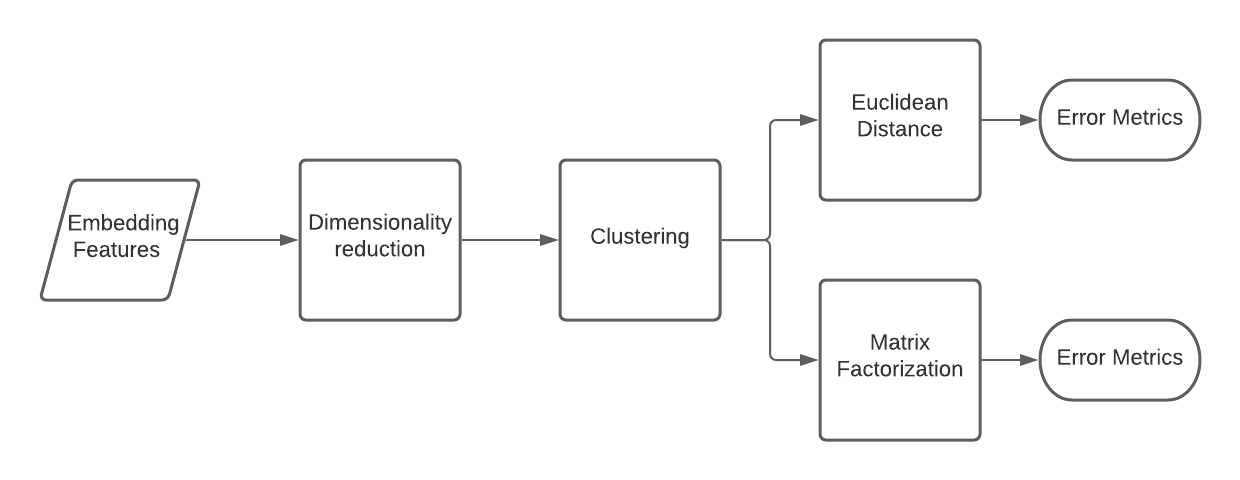
\includegraphics[width=0.9\textwidth]{images/experiment.png}
    \caption{Proposed validation method}
    \label{fig:method_architecture}
\end{figure}

The dataset of choice in order to test its techniques was  \textit{globo.com dataset} from \cite{deSouzaPereiraMoreira:2018:CDL:3240323.3240331} 
that aggregates streams of user clicks with more than 2.8 millions of clicks.

%TODO Deve ser atualizado
On chapter 3 the concepts, history and motivation of choice on used algorithms are presented. Chapter 4 presents the problem and the solution definition.
At the Fifth chapter, experimentation is revealed as its used tools, metrics are applied in order to measure accuracy and reliability of the proposed techniques.

% =======================================================================

\chapter{Theoretical Background and Related Work}
On this chapter the foundations for this work will be introduced.

    \section{Basic concepts}
    At the current section it will be presented the basic building blocks, those are crucial to assemble the complete picture of this work, the concepts presented at its pipeline order are such as \(user\), \(account\), \(item\), \(session\) and \(recommendation\ systems\).
        
        % TODO explain each item
        % User and Account
        Account is the common gateway for an user to access the platform content, most of past works consider that each account is in fact one user which may happen on most scenarios because normally each user has its own account, but sometimes and even more on paid platforms, an account is shared between more users.
    
        % Item and Session
        An item is a pair with a click timestamp and a media id identification. 
        At Globo dataset, each item is a  set \((timestamp, click\_id)\) but 
        in any other dataset, the click id is a reference to news, music, 
        image, video or any metadata associated. A session is a well defined 
        segment from a stream of items from one account. There are many ways 
        of defining session boundaries, on \cite{10.1145/362883.362920} the session 
        is defined by using time threshold, same as \cite{10.1145/2736277.2741117}. 
        For example when a user stays inactive for an amount of time, that can be 
        considered an end of a session and start of another. In this proposal the 
        sessions will be split considering the content type in order to identify 
        account sharing or even user profiling for different user tastes.

    \section{Basic methods}
    Here the methods for manipulating the just presented basic blocks will be briefly described, such as \(recommendation\ system\), \(dimensionality\ reduction\) and \(clustering\).
    
        \subsection{Recommendation system}
        The role of a \textit{recommendation system} is to make inferences of new \(items\) that the \(user\) would like and suggest them. It is a set of algorithms that together they can return for example an ordered list of probability/similarity from items that were previously compared against other items. These other items must be similar from the ones that the \(account\) have interacted or similar accounts have interacted with.
        Variables such as click-rate, visit frequency, time spent on page can be considered to calculate an affinity between interacted \(items\) and \(account\).

        A recommendation system can have four main classifications:
        \begin{itemize} 
            \item Implicit vs Explicit
            \item Content-based vs Collaborative
        \end{itemize}

        \textit{Implicit vs Explicit} definitions correspond to the way data is semantically related between the pair \(account\)-\(item\). On \(Implicit\) recommendation systems there is an implicit relationship between the used item and the expectation that the majority of those items are desirable by its user, on the other side of the spectrum, there are the \(Explicit\) recommendation systems that usually uses a rate system given by the \(user\), so there is not just a simple link between both entities, but also a subjective magnitude that could be either positive or negative, qualitatively speaking.

        \textit{Content-based vs Collaborative} classifies on an \(account\)-\(account\) relationship. On the first one the similarity between interacted items on a same account is used to retrieve similar new items that the user didn't yet explored, on the second one, the comparison is based upon other accounts that share similarity, so items from these accounts that are missing on the interaction history can be recommended. On state of art systems, both methods are combined in order to get the best results.    

        \subsection{Dimensionality reduction}
        The more dimensions a dataset has the more diluted the statistical significance becomes, 
        because data sparsity grows exponentially as the dimensions grow linearly, 
        this phenomena is called \textit{the curse of dimensionality} and is described on \cite{10.1093/imamat/24.1.59} and one on way to finding statistical significance are techniques of \textit{dimensionality reduction}.
        One of firsts successful algorithms is called \textit{Principal Component Analysis}, 
        its model was developed in 1933 by \cite{hotelling:33} and it consists in finding linear combinations between pair of dimensions that corresponds to most statistical significance trough standard deviation metrics, where the two most significant linear combinations becomes the main dimensions and its points are plotted in a two dimensional Cartesian plane.
        Those techniques are used before applying Clustering algorithms, because normally media contents are described as an array of multidimensional features. 
        
        \subsection{Cluster analysis}
        It is the method for grouping items that share a vicinity/similarity and then labelling each one of the groups, normally, clustering algorithms are applied on points plotted on two-dimensional planes. There are many types of algorithms for classifying clusters, such as \textit{distribution-based}, \textit{density-based}, \textit{centroid-based}, \textit{connectivity-based} and others. In this work the centroid-based algorithm \(Affinity\ propagation\) was used for classifying clusters of similar \(items\), in this case each \(item\) represented by one news content.

% =======================================================================
% More related works
\section{Related works}
% This chapter will present previous works that used user identification and sessionization as solution, both profile-level and time-level methodologies.
        
    \subsection{Time-level user identification}
    The work \cite{10.1145/2736277.2741117} consists in monitoring different domains of online activity browsing (Games, search engines, page views), thus achieving session identification using a fixed 30 minutes inactivity threshold as session identification, authors demonstrates high regularity between different sessions from a same user. 
    Since they do not address account sharing, there is a chance that threshold based on item usage or user behaviour and not on time usage, would have more impact on identifying sessions related to different users.
    On \cite{JINDAL2020} et al, they propose a dynamic threshold heuristic based on user behaviour history, their discoveries show that short time user navigation are more often and less correlated than longer ones, making them easier to categorize and achieving a higher accuracy. However, this method apply a threshold into the user behaviour pattern, and differently, this work relies on the distance between topics inside a session, also the proposed method uses fixed threshold for simplicity reasons.

    \subsection{Profile-level user identification}
    One of the state of art contribution is from \cite{Jiang:2018:IUB:3209978.3210054} that using the \textit{LastFM} and \textit{KKBOX} datasets, they address a solution on user identification on shared accounts at streaming platforms given its history logs, proposing the novel unsupervised learning named SHE-UI. They could be able to identify groups of users sharing a same account, bringing their solution to an user-level recommendation domain instead of account-level.
    A problem that e-commerce recommendation systems face is when an advertisement of an exact size or individual characteristic for an user is required, because other users may end up contaminating the account history and spoiling the estimate of these unique attributes or sizes, on \cite{10.1145/3178876.3186149} et al the problem is discussed using Amazon.com e-commerce, instead of dealing with each account as a specific user and single profile, they propose a multi-persona approach boosting the accuracy, however, this method does not work well on products that have a high variability on its characteristics.

% Aqui tá faltando trabalho relacionado.
% =======================================================================

\chapter{Methodology}
At the current chapter, problem definition, algorithms, tools used for the proposed methods and its validations are discussed and presented with its motivations.

    \section{Problem definition}
    Let \(I \) be a set of items where \(i \in I \) and an item \(i\) represents a news. Let a set of users \(U\) where \(u \in U \) and each user \(u\) does not repeat itself into the set.
    A session \(s\) is defined by a list of items \(s_{1} = \{i_{1}, i_{2}, i_{3}\}\) and belongs to an individual user \(u_{1}\), the items may repeat inside a session and also between sessions.
    It is considered by definition, that each User is an account itself, and that most of users doesn't share its account, and the amount of shared accounts have low  statistical significance into the end result.
    
        \subsection{Simulated Accounts and Sessions}
        In order to simulate a shared account, two sessions are concatenated into a new session as \(s_{1} = \{i_{1}, i_{2}, i_{3}\}\) and  \(s_{2} = \{i_{7}, i_{8}, i_{9} ...\}\) and those sessions must belong to different users.
    
        the new simulated session consists in the following representation
    
        \(s_{12} =  s_{1} \cup  s_{2} =  \{i_{1}, i_{2}, i_{3}, i_{7}, i_{8}, i_{9}, ...\}\)
    
        The objective of the proposed method is to identify the exact frontier-item between sessions and revert this concatenation process separating the new session  \(s_{12}\) into the original \(s_{1}\) and \(s_{2}\) sessions, in that scenario, item \(i_{3}\) would be the frontier-item, since it is the last item of the first session \(s_{1}\).
    
        This process should use only the item content or category as parameters, being blind to the user ids or timestamps.    
        % Organizar os trabalhos relacionados entre:
        
        % Secão 2.1: Investigações que dependem da identificação de sessões online de usuários. Aqui entra, por ex., o trabalho de Jiang et al. (2017). 
        
        % Secão 2.2: Investigações que discutem possíveis técnicas para quebrar sessões online dos usuários.
        
        Time-based sessions are the most commonly used as consensus as a method for example at \cite{10.1145/3184558.3191582} it is used a defined session trough a fixed time, but the way they make it flexible, were by using a decaying time-based weight into the session items, they used this approach to overcome the short life-span of news. At the proposed method, since not the news itself, but it's topic, the short life-span problem wasn't expected to be relevant enough.
    
        \subsection{Cold start problem}
        This is a flaw of content-based recommendation systems, since it is content-centric, when an user is fresh having little or no content history, the method lacks on precision. 
    
        A Collaborative system, is no different in terms of this flaw, but it is more resistant, since it collaboratively uses content history from other users, it can fill the gap against data scarcity from fresh users.
        
        In order to avoid this dilemma, the proposed metrics are based on previously filtered sessions, where the first method use sessions with more than 10 items, and the second method, more than 200 items.
    
        % Matheus: Necessário? na introdução este problema é brevemente descrito e seu autor citado é o motivo do uso de um algoritmo como o TSNE.
        \subsection{Curse of dimensionality Problem}
        Because content analysis and classification requires a complex analysis that generates great amounts of features/dimensions, the curse of dimensionality is very relevant as a problem, any media should be translated into a multi dimensional space before the classification.
        
        A successful and recent example of PCA use is on the physical simulation from a 3D engine at \cite{10.1145/3309486.3340245}. Before a complex process of vector computation for physics simulation, PCA was used to minimise the information-trash creating a meaningful and denser subspace in terms of information relevance before training a neural network, making the algorithm 10X faster and using less memory.

        
    \section{Algorithms and Datasets}
    
    On this section, all the datasets and used algorithms will be described as well as it historic evolution against their pioneers.
    
        % O objetivo desse capítulo é apresentar os conceitos e algoritmos necessários para a construção da metodologia de avaliação....
        
        % Iniciar todos os capítulos com uma descrição do que é o conteúdo do capítulo. Por exemplo, nesse capítulo serão apresentados os conceitos e recursos que irão compor a metodologia de avaliação da eficácia e eficiência das técnicas para separação das sessões online de usuários. A seção organiza a discussão dos conceitos e recursos entre aqueles que foram usados no trabalho e aqueles que não foram usados. Em ambos os casos, será feita uma discussão sobre as potencialidades do conceito, no caso em que são usados, ou das limitações que impedem a aplicação dos mesmos, nos casos em que não são utilizados.
        
        % Possível organizaçao das seções:
        % 3.1. Caracterização do Traço do Globo.com
        % Quantos registros eles tem, quantos usuários, qual o tamanho, qual o período que eles refletem, qual a natureza deles, quais os campos que cada entrada possui... 
        
        % 3.2. Técnicas Utilizadas
        % 3.3. Técnicas Não Utilizadas
    
        % Matheus: Sinto que preciso reduzir este texto, visto que não usei PCA e ele tem valor apenas explicativo
        \subsection{Principal Component Analysis} 
        Principal Component Analysis is the first known form of dimensionality reduction on multidimensional data.
        Its model was developed in 1933 by \cite{hotelling:33} and the main idea of its technique is finding linear combinations from pairs of dimensions that corresponds to most statistical significance trough standard deviation metrics in each one.
        So, imagine you have N dimensions and M items with its coordinate in this space, PCA would translate this N-space matrix into another N-space matrix trough rotations on those dimensions, based on standard deviation metrics finding the biggest deviation in each linear combination. 

        Since each linear combination is a pair of dimensions, the best angular coefficients to represent the new rotated dimensions are calculated using Least Squares Regression, fitting the points in this two dimensional sample relation, making the the line span represents a new dimension with the biggest standard deviation possible, meaning a better statistical significance.
        After this process, a rank of standard deviations called \textit{scree-plot} is made trough all those new rotated dimensions, and the two most significant dimensions, with bigger deviations, will better represent the data in a 2-dimensional Cartesian fashion.

        In Fact, the diagonal of the resulting matrix of the whole process is the variance of each dimension ordered by statistical significance and it is the \textit{scree-plot}.

        However, this is the naive approach in data dimensionality reduction, but it is very useful when data have information linked trough linear relations.
        A successful and recent example of PCA use is this physical engine in \cite{10.1145/3309486.3340245}, that before a complex process of vector computation for physics simulation, a PCA was used to reduce the "information-garbage" creating a meaningful and denser subspace in terms of relevant information before training a neural network, making the algorithm 10X faster using less memory.
        
        In the example of globo dataset, as \cite{deSouzaPereiraMoreira:2018:CDL:3240323.3240331} mentions, they could not provide the globo news content, since it is closed source, however, they mention in their article also, that TSNE would represent a better representation of the reduced data, since this matrix have non-euclidean information relationships, so in that case, PCA would not fit the best 2-dimensional surface in terms of statistical significance.
        To think what would happen using a excessively linear algorithm like PCA to find the best surface, imagine a zig-zagged bent bread and you want to cut the middle of it with a knife, PCA would make a straight line cut ignoring the format of the bread. In that case, the algorithm they recommend is TSNE, a modern and state-of-art technique for dimensional reduction that uses machine learning and gradient descend techniques.
        \newline
        
        \subsection{TSNE, a state-of-art dimensionality reduction}
        As any other algorithm for this purpose, it maps highly dimensional data into a low dimensional representation resuming the data and resisting against dimensionality curse as mentioned \cite{10.1093/imamat/24.1.59}, but differently from PCA, TSNE is a non-linear method, proposed in 2008 by \cite{vanDerMaaten2008}, this method preserves local geometry and deform global geometry, more specifically, it tends to clump points that share a near neighborhood making the clusters more evident.
        Non-linear means that if you have highly dimensional data that has a geometric representation of a curvy non-convex surface of points, for example, PCA due to its linearity would make a straight cut into this curve finding straight planes and never really fitting into the curvy surface, PCA has its algorithms variances that reduce its problems, like the Kernel PCA, but TSNE is considered to be the state-of-art for reasons below.

        TSNE It is a sequel of SNE (Stochastic Neighborhood embedding), but because the current distribution from SNE not only hardly clump the points close to each other but it is use to be computationally slow, because of the use of exponentiation when calculating the distribution equation.
        The "T" letter stands for T-student distribution, it is computationally faster and has a less severe penalty on point agglutination due to its natural flattened curve, thus winning the "state-of-art" title due to its low cost and better precision.

        On the figure below, there is the result of TSNE on Globo dataset highly dimensional embedding that represents the content of each news, this exactly plot and its data was used on the proposed method, each point represented below is a relationship of a Xs, Ys coordinate with an article id 
        \par
            \begin{figure}
                \centering
                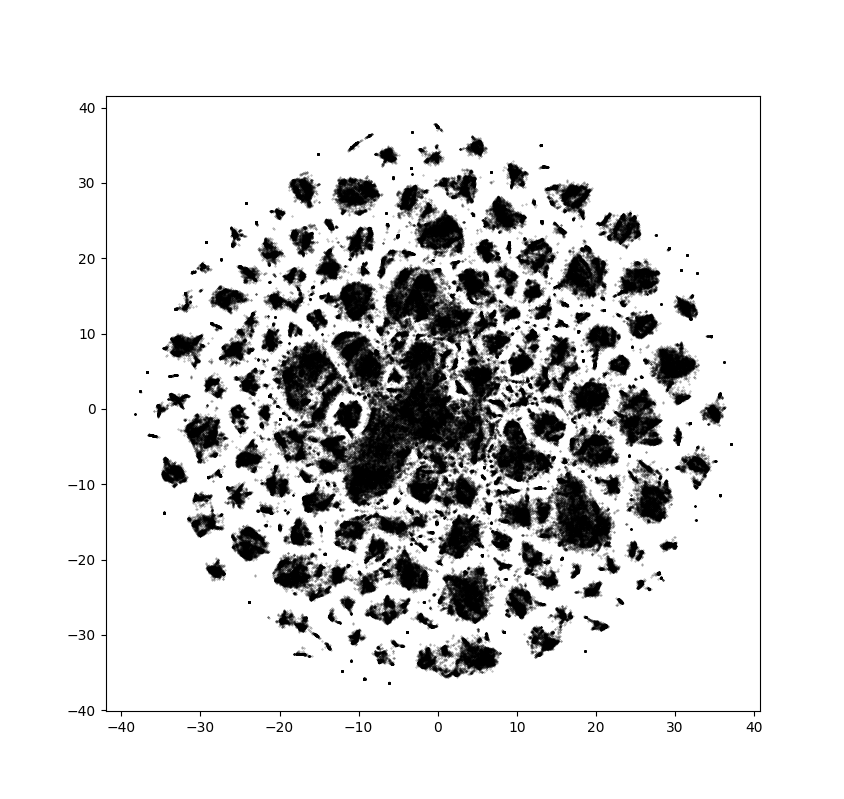
\includegraphics[width=0.8\textwidth]{images/tsne_clusters.png}
                \caption{TSNE plot}
                \label{fig:tsne_plot}
            \end{figure}
        
        \subsection{Clustering with Affinity propagation}

        The advantage of affinity propagation between other algorithms is that it does not need to specify an estimate of quantity of points found into the space, it naturally walks trough the points and finds the resulting clusters.

        On the image below there is the visualization of the discovered clusters on the low dimensional embedding representation from TSNE result, and on the second image, the center of each cluster representing a topic, that later should be used to calculate the semantic difference from each topic based on the euclidean distance from the pair of topics being compared.
         
            \begin{figure}
                \centering
                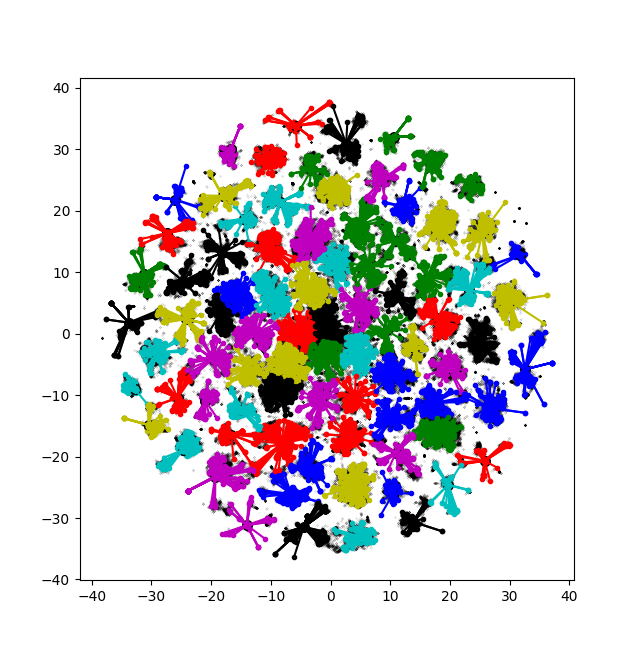
\includegraphics[width=0.8\textwidth]{images/affinity_plot.png}
                \caption{Affinity propagation and each news relating to its cluster}
                \label{fig:affinity_propagation_clusters}
            \end{figure}
            
            \begin{figure}
                \centering
                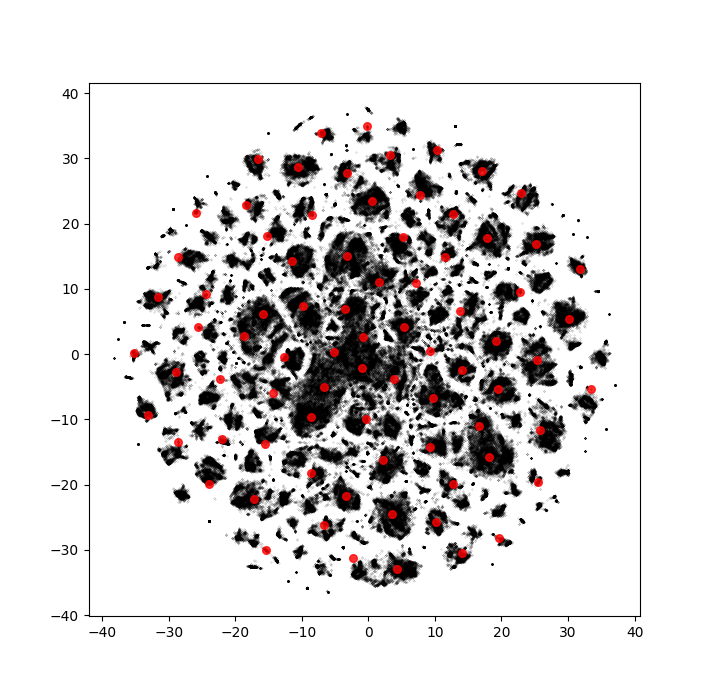
\includegraphics[width=0.8\textwidth]{images/tsne_clusters_plot.png}
                \caption{Affinity propagation topic clusters}
                \label{fig:affinity_propagation_centers}
            \end{figure}    
    
        \subsection{Matrix Factorization}
        Netflix is known for it's competitions for collaborative filters algorithms and in 2008 one algorithm called matrix factorization  achieve a huge breakthrough in collaborative filtering algorithms, and it is like the prime factors for grown ups, or in other words, using matrices as factors instead of prime numbers, it is a useful mechanism to separate the users-items matrix into a items matrix and a user matrix, that their multiplication result in the original \(users-items\) matrix, results into Item X User original association matrix that each item is the relation of one user to a single item.
        The usefulness of this factorization, is that since the original matrix is sparse, because not every user in its history has real relation with every item, you can fill the missing values by making inferences on the factorized data.
        An optimal way of doing so is by using the Alternate Least Squares algorithm explained below that uses Gradient Descent as convergence algorithm.
        
        \subsection{Alternate Least Squares}
        Alternate Least Squares, is a faster variant of the Matrix Factorization that allows it to be computational distributed, the as matrix factorization, it has SVD as central role on the factorization between item and user matrices, but in this case, a cost function with an error function is alternated between each matrix, updating the elements of one matrix at a time, this computational behaviour reduces the complexity of the cost function and allows it to be computed in a distributed fashion.
        Today a common implementation of ALS is from Spark \(Hadoop\) in java, but also have facade libraries that allow calling ALS from spark \(Hadoop\) from other languages like Scala and Python (Pyspark).

    \section{Technology usage}

        \subsection{Python and its libraries}
        It was used \(Python3\) with \textit{pandas} \cite{reback2020pandas} and \textit{numpy} as main data manipulation, \(Pyspark\) was used for ALS method recommender system. 
        \(Pyspark\) is a python library that is a facade for a java spark hadoop spark application server that uses map/reduce in order to make distributed computations.
    
        For TSNE and Affinity propagation \(sklearn\) library was the choice.
        
        \subsection{Applying Dimensionality reduction}
        Because Globo news text data is closed source, \cite{deSouzaPereiraMoreira:2018:CDL:3240323.3240331} made available the trained article embeddings data \footnote{https://www.kaggle.com/gspmoreira/news-portal-user-interactions-by-globocom} generated from its unique \textit{CHAMALEON} RNN-based algorithm. The embedding file consists into a matrix of 250 dimensions of features and 364,047 news articles, those features are a representation of the content for each respective news article.
    
        On the proposed method only the following data and respective embedding were considered: \textit{click\_timestamp, article\_id} and \textit{{}user\_id}.
        
    
        Since on their work TSNE was mentioned as a good method for dimensionality reduction, TSNE was applied on the embedding, resulting into a pair of coordinates X, Y for each article id as the dataframe sample below:
        
        \begin{table}[!ht]
            \centering
            \begin{tabular}{ |c|c|c| } 
                \hline
                article\_id & x & y \\
                \hline 
                ... & ... & ... \\
                69 & 10.950659 & -26.211418 \\ 
                81 & 34.414822 & -0.690890 \\ 
                84 & 35.335995 & -1.578238 \\ 
                ... & ... & ... \\
                \hline
            \end{tabular}
            \caption{TSNE coordinate results}
            \label{tab:tsne_results}
        \end{table}
        
        \subsection{Applying Clustering}
        At this step, \textit{Affinity propagation} is applied on the TSNE result data plane, several damping parameters were tested and presented further at the error metrics section. 
        After the clustering, each cluster center point into the resulting plane receives a human-readable label, the image below shows a distribution of consumed topics by a sampled user resembling a 
        Benford's law distribution:
        \newline
        
        \begin{figure}[!ht]
            \centering
            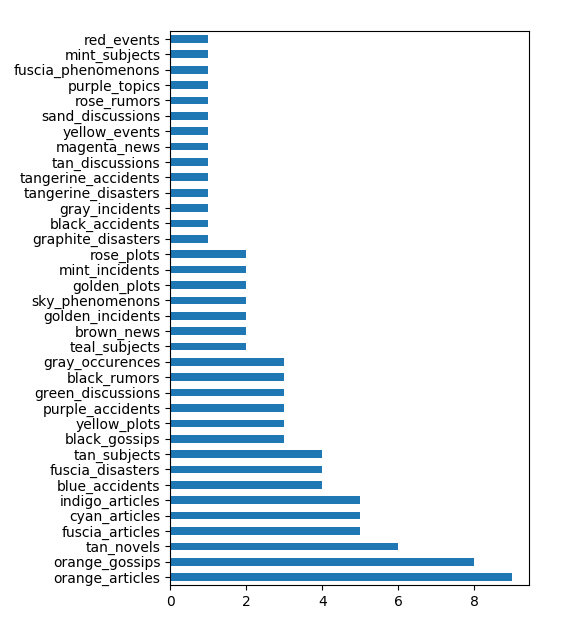
\includegraphics{images/frequencies.png}
            \caption{Topic frequencies from a sampled user}
            \label{fig:topic_frequency}
        \end{figure}
        
    
        further, this data will be used into session items and used on both methods euclidean distance and ALS methods.
        
        \begin{table}[!ht]
            \centering
                \begin{tabular}{ |c|c|c| } 
                \hline
                x & y & label \\
                \hline 
                ... & ...  & ... \\
                19.699291 & -28.117729 & tangerine-events \\ 
                -8.711248 & 21.906485 & purple-occurrences \\ 
                11.325381 & 3.893677 & yellow-episodes \\ 
                ... & ...  & ...  \\
                \hline
                \end{tabular}
            \caption{Labeled cluster centers}
            \label{tab:labeled_clusters}
        \end{table}

% =======================================================================

\chapter{Results}

    Here there will be a comparison between \(euclidean\ distance\) threshold against \(alternate\ least\ square\) methods and its parameters variations.

    \section{Globo.com dataset} %TODO contextualização disso nesse capítulo
    It is a collection that consists on the following:
    \begin{itemize}
        \item approximately 2.8 millions news clicks
        \item more than 300 thousand users
        \item 45 thousand news articles
        \item 250 dimensional feature matrix
    \end{itemize}
    
    Since the access to articles text data were not allowed by the company for commercial reasons, at \cite{deSouzaPereiraMoreira:2018:CDL:3240323.3240331} presented CHAMELEON, a RNN algorithm for feature extraction, and together with the dataset, they allowed the use of an feature embedding file extracted from its novel algorithm. Every news from the dataset have its own 250 feature dimensions on the embedding matrix
    
    The dataset consists on the following data for each click as the columns:
    \newline \textit{user\_id, session\_id, session\_start, session\_size, click\_article\_id, click\_timestamp,}
    \newline \textit{click\_environment, click\_deviceGroup, click\_os, click\_country, click\_region,}
    \newline \textit{click\_referrer\_type} 

    sample showed on the table below
    
    \begin{table}[!ht]
        \centering
        \begin{tabular}{ |c|c|c|c|c|c|c|c|c|c| } 
            \hline
            click\_timestamp & user\_id & article\_id & click\_country & click\_region & ... \\
            \hline 
            ... & ...  & ...  & ...  & ... & \\
            1506826800026 & 59 & 234853 & 1 & 21 & \\ 
            1506826801702 & 79 & 159359 & 1 & 13 & ...\\ 
            1506826804207 & 154 & 96663 & 1 & 25 & \\ 
            ... & ...  & ...  & ...  & ... & \\
            \hline
        \end{tabular}
        \caption{Globo dataset sample as Dataframe}
        \label{tab:globo_dataset_sample}
    \end{table}

    \section{Euclidean Distance as threshold}

        \subsection{Error metrics}
        \begin{itemize}
            \item The cutoff is a row index that belongs to one of the sessions, this index is found by a cutoff trigger heuristic
            \item Because the two sessions doesn't have the same amount of items, thus asymmetric, a normalization of the error metric is constructed.
            \item It is calculated the difference between the number of items from the inferred index(found by heuristic) and the perfect index(the real cutoff) and divided by the total number of items at the artificial session (made by two real sessions), as represented above in this colorized table by the error column:
            
            \begin{table}[!ht]
                \centering
                \begin{tabular}{c|c|c}
                    \hline
                    \rowcolor[RGB]{239,239,239}
                    index & user\_id & error \\
                    \hline 
                    \rowcolor[RGB]{140,140,140}
                    0 & 111 & 1 \\ 
                    \rowcolor[RGB]{197,197,197}
                    1 & 111 & 0.66 \\ 
                    \rowcolor[RGB]{226,226,226}
                    2 & 111 & 0.33 \\ 
                    \rowcolor[RGB]{255,255,255}
                    3 & 888 & 0 \\ 
                    \rowcolor[RGB]{239,239,239}
                    4 & 888 & 0.16 \\ 
                    \rowcolor[RGB]{222,222,222}
                    5 & 888 & 0.33 \\ 
                    \rowcolor[RGB]{206,206,206}
                    6 & 888 & 0.5 \\ 
                    \rowcolor[RGB]{189,189,189}
                    7 & 888 & 0.66 \\ 
                    \rowcolor[RGB]{173,173,173}
                    8 & 888 & 0.83 \\ 
                    \rowcolor[RGB]{140,140,140}
                    9 & 888 & 1 \\ 
                    \hline
                \end{tabular}
                \caption{Desired cutoff example gray-colored by error}
                \label{tab:cutoff_table}
            \end{table}
            
            So in this example, the index 3 is the perfect cutoff, representing the real threshold between the two sessions, the picked index by the cutoff heuristic, will receive the respective error from its index row.
        \end{itemize} 
        
        % TODO subseção com apenas 1 parágrafo
        \subsection{Affinity propagation parameters variation}
        The damping parameter was fixed at 0.9,
        15 cutoff values were tested between values 1 and 60, linearly spaced for each iteration with a different cutoff, 
        The output was a vector of error values of the same size of the simulated sessions(one for each session, about 32 thousand sessions).
        Then, from this error vector, it was calculated its mean and standard deviation for each iteration (15 iterations), so that we could measure its reliability and precision.
        
        % TODO subseção com apenas 1 parágrafo
        \subsection{Sessions simulation}
        Because the dataset already have user ids in each row, it was considered that the majority of accounts were in fact from individual users, in that case, the hypothesis is that even if some users really shared the same account, this would be statistically irrelevant when analyzing the whole dataset.
        Considering that scenario true, the simulated sessions is constructed as a concatenation of two streams of two separated user ids.
        as addressed below a sample from a simulated session:
        
        \begin{table}[!ht]
            \centering
            \begin{tabular}{ |c|c|c|c|c|c| } 
                \hline
                \  & click\_timestamp & user\_id & x\_centroid & y\_centroid & distance \\
                \hline 
                 ... & ... & ... & ... & ... & ... \\
                 7 & 1507630999019 & 6207 & -8.487595 & 21.294018 & 22.376601 \\
                 8 & 1507854592096 & 6207 & -18.733793 & 3.206146 & 20.788355 \\
                 9 & 1507854731273 & 6207 & 9.636348 & 0.610321 & 43.517998 \\
                 10 & 1507854761273 & 6207 & -18.733793 & 3.206146 & 43.517998 \\
                 11 & 1507987156229 & 6207 & -8.487595 & 3.206146 & 43.517998 \\
                 12 & 1507988999717 & 6207 & 3.864952 & -3.751176 & 27.925744 \\
                 13 & 1507989029717 & 6207 & 5.004131 & 3.442250 & 7.283071 \\
                 \rowcolor[RGB]{220,220,220}
                 14 & 1507061447189 & 143259 & 25.503668 & -1.358489 & 21.054171 \\
                 15 & 1507061615464 & 143259 & 18.530073 & -15.994876 & 16.212799 \\
                 16 & 1507061615464 & 143259 & 18.530073 & -15.994876 & 0.000000 \\
                 17 & 1507160861114 & 143259 & -8.914310 & -9.236862 & 28.264199 \\
                 18 & 1507160984701 & 143259 & 3.675873 & -24.894243 & 24.050260 \\
                 ... & ... & ... & ... & ... & ... \\
                \hline
            \end{tabular}
            \caption{Simulated session sample}
            \label{tab:session_simulation}
        \end{table}
        
        \begin{table}[!ht]
            \centering
            \begin{tabular}{ |c|c|c| } 
                \hline
                cutoff & mean & std \\
                \hline 
                1.00 & 0.6934 & 0.2441 \\ 
                5.21 & 0.6871 & 0.2511 \\ 
                9.42 & 0.6677 & 0.2704 \\ 
                13.64 & 0.6537 & 0.2816 \\ 
                17.85 & 0.6336 & 0.2964 \\ 
                22.07 & 0.6140 & 0.3104 \\ 
                26.28 & 0.5999 & 0.3196 \\ 
                30.5 & 0.5956 & 0.3281 \\ 
                34.71 & 0.600 & 0.3360 \\ 
                38.92 & 0.6259 & 0.3449 \\ 
                43.14 & 0.6707 & 0.3479 \\ 
                43.35 & 0.7456 & 0.3347 \\ 
                51.57 & 0.7949 & 0.3156 \\ 
                55.78 & 0.8607 & 0.2765 \\ 
                60.00 & 0.9272 & 0.2118 \\ 
                \hline
            \end{tabular}
            \caption{Cutoff testing}
            \label{tab:cutoff_sample}
        \end{table}
        
        % TODO subseção com apenas 1 parágrafo
        \subsection{Distance calculation}
        It represents how different two topics are.
        In a session dataframe, it is the euclidean distance between the cluster centroid coordinates from the current index N, with the coordinates from the centroid of the N-1 index. 
        
        % TODO subseção com apenas 1 parágrafo
        \subsection{Cutoff criteria}
        It is used a arbitrary threshold as cutoff, when the metric (distance or ALS prediction) is found above this threshold, it is considered a different session from a different user   
        
        \begin{table}[!ht]
            \centering
            \begin{tabular}{ |c|c|c|c| } 
                \hline
                article\_id & x & y & label \\
                \hline 
                ... & ... & ... & ... \\
                69 & 10.950659 & -26.211418 & magenta-episodes \\ 
                81 & 34.414822 & -0.690890 & orange-accidents \\ 
                84 & 35.335995 & -1.578238 & orange-accidents \\ 
                ... & ... & ... & ... \\
                \hline
            \end{tabular}
            \caption{Labeled article coordinates}
            \label{tab:article_coordinates_table}
        \end{table}
        
        \newpage 

        \subsection{Heatmaps}
    
        The heatmaps error results are interpreted as the following:
        \begin{itemize}
            \item The Vertical axis of the represents the affinity propagation damping factor
            \item The Horizontal axis corresponds to the chosen cutoff distance threshold
            \item the value of each item on the heatmap corresponds to one of two metric errors: Mean error, Standard deviation error.
        \end{itemize}
    
        The objective of this metric is find a lower than 50\% mean error and the biggest ratio Mean over Standard Deviation. 
    
        In that case a low mean and a low std. is desired.
        
        \begin{figure}[!ht]
            \centering
            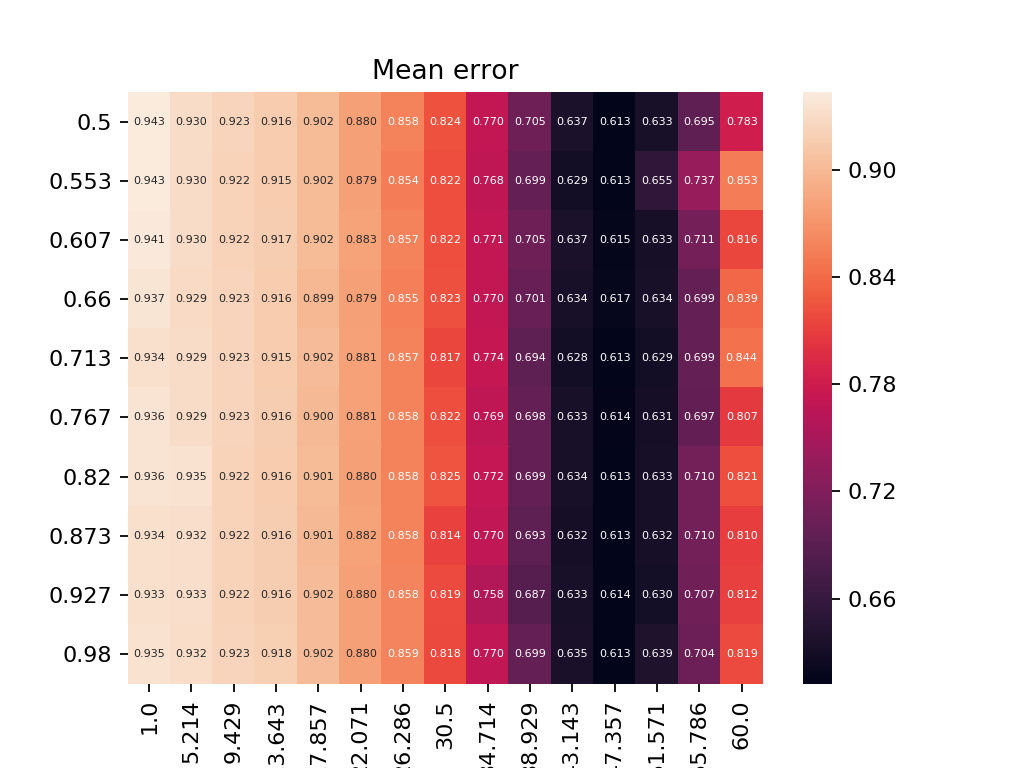
\includegraphics{images/error_mean.png}
            \caption{Error mean heatmap}
            \label{fig:error_mean_heatmap}
        \end{figure}
        \par
        
        \begin{figure}[!ht]
            \centering
            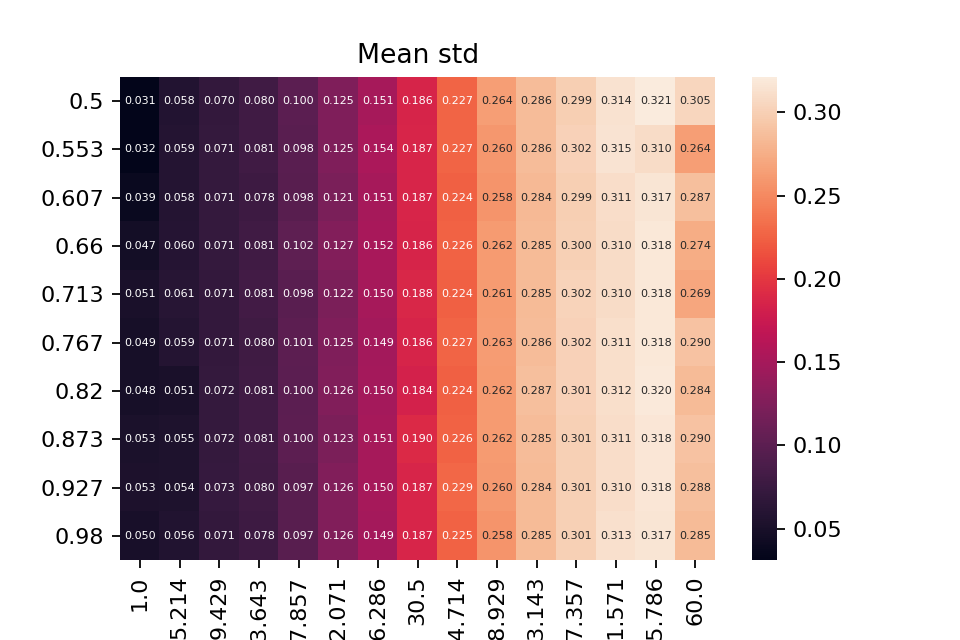
\includegraphics{images/error_std.png}
            \caption{Error standard deviation heatmap}
            \label{fig:error_std_heatmap}
        \end{figure}
        
        \newpage 
    
    \section{Applying alternate least squares}
        \subsection{Method}
        In order to avoid cold start, only users with more than 200 items in total were chosen.
        Like in the Euclidean Distance experiment, fictitious sessions were created, but instead of distance column as error metric, a new column 'prediction' were added that corresponds to the predicted probability that one user have to read that article, the chosen user is the user of the first session.
        

        The expected result is that, on the first session, the prediction should have low standard deviation and a high mean, and on the second session, using the firsts session user\_id, as prediction parameter, the expected mean, in case of different user styles, should be lower and also the standard deviation.
        
        \newpage 
        
        % TODO subseção com apenas 1 parágrafo
        \subsection{Error Metrics}
        The following table was created as result:
        \begin{table}[!ht]
            \centering
            \begin{tabular}{ |c|c|c|c| } 
                \hline
                user\_id & user\_id\_to\_predict & prediction\_mean & prediction\_std \\
                \hline 
                413 & 413 & 0.83287 & 0.2799 \\
                45502 & 413 & 0.86549 & 0.25900 \\
                \rowcolor[RGB]{220,220,220}
                12897 & 12897 & 0.84201 & 0.3291 \\
                \rowcolor[RGB]{220,220,220}        
                16695 & 12897 & 0.91515 & 0.27717 \\
                2930 & 2930 & 0.79370 & 0.34552 \\
                9261 & 2930 & 0.87126 & 0.2551 \\
                \rowcolor[RGB]{220,220,220}        
                20001 & 20001 & 0.8777 & 0.24580 \\
                \rowcolor[RGB]{220,220,220}        
                6344 & 20001 & 0.91090 & 0.2383 \\
                62025 & 62025 & 0.75506 & 0.35445 \\
                19864 & 62025 & 0.47764 & 0.27196 \\
                \rowcolor[RGB]{220,220,220}        
                43017 & 43017 & 0.83342 & 0.27467 \\
                \rowcolor[RGB]{220,220,220}        
                21356 & 43017 & 0.81031 & 0.28030 \\
                3391 & 3391 & 0.85998 & 0.2949 \\
                681 & 3391 & 0.87366 & 0.30739 \\
                \rowcolor[RGB]{220,220,220}        
                11521 & 11521 & 0.61621 & 0.3742 \\
                \rowcolor[RGB]{220,220,220}                
                59193 & 11521 & 1.01384 & 0.5024 \\
                11359 & 11359 & 0.88445 & 0.2596 \\
                23036 & 11359 & 0.91379 & 0.24409 \\
                \rowcolor[RGB]{220,220,220}                
                22301 & 22301 & 0.81135 & 0.30362 \\
                \rowcolor[RGB]{220,220,220}                
                77985 & 22301 & 0.78393 & 0.32523 \\
                13885 & 13885 & 0.85638 & 0.264 \\
                9193 & 13885 & 0.80591 & 0.2890 \\
                \hline
            \end{tabular}
            \caption{Alternate Least Squares measurements}
            \label{tab:alternate_least_squares_metrics}
        \end{table}
        It was extracted metrics from 413 users

% =======================================================================

\chapter{Conclusion}
The standard deviation presented on the heatmaps with different input parameters reveals that the euclidean distance as threshold method does not have enough precision, but these results could have many explanations for this lack of precision not only from the method itself. Since globo dataset is closed source and the features available from \cite{deSouzaPereiraMoreira:2018:CDL:3240323.3240331} were created from his own algorithm, a certain level of belief was implied that the features really reflected its content and his algorithm worked well on quantitatively describing them.

Another possible cause could be the dimensionality reduction step, no other algorithm was tested but the recommend TSNE from \cite{deSouzaPereiraMoreira:2018:CDL:3240323.3240331}.

Finally, news as a type of media have a chaotic nature, even when readers have his preference for certain topics, unexpected and relevant news from other topics may arrive and catch the readers eyes those phenomena, maybe they are common and can hinder this method of session cut by euclidean distance threshold. 

\bibliographystyle{packages/abntex2-alf}
\bibliography{biblio}

\end{document}
